% Drawing 83/11-5 -- folder 83, batch 11, archive page 208 (PDF page 209).
% Transcription: Deux cubes en perspective. Sur le petit, en haut à gauche, les arêtes portent $a$, $b$, $c$, $d$, $a'$, $b'$ et, en dessous, $a+\alpha$, $b+\alpha$, $c+\alpha$, $d+\alpha$. Sur le grand, les arêtes portent, cerclées, $a$, $b$, $c$, $d$, $u$, et $a+\alpha = a'$ (cerclé $a'$), puis $b+\alpha$, $c+\alpha$, $d+\alpha$, $u+c-a$ ; sur une face : $v = u - (d-b)$ (signe surchargé).
% Kind: two cubes with edge labels. Method 2 (schematic redraw from the facsimile). Status: partial.
% Notes: Small cube (top left) on eight computed corners: front face a (top), a' (left), b' (right, heavy, doubled in ink), the bottom edge; receding edges d, b and the back edge c on top; the back right vertical, the bottom right receding edge, and the three hidden edges (thin) meeting at the back bottom left corner. Labels at \small as he placed them: c, d, a, b, a', b', and below d+alpha, c+alpha, b+alpha, a+alpha. Large cube on computed corners: front face with the top edge (circled a), the left vertical (circled u, ending in an arrowhead before the bottom corner, as on the page), the right vertical and the bottom edge (a+alpha = circled a'); top receding edges (circled d on the left one, circled b on the right one) and the back top edge (circled c), meeting at the back corners; back right vertical; bottom right receding edge (b+alpha); the hidden back bottom edge (c+alpha), the short hidden stroke from the front bottom left corner (d+alpha) and a short fragment of the hidden left vertical. Inside: u+c-a, v = u-(d-b) (the sign before (d-b) is overwritten), and v+(c-a) = u at the right. Still differs: the hidden back left vertical is not drawn on the page except for one fragment, so its corner is computed from the two drawn edges; the overwritten mark by c+alpha in the small cube and the stray dots and ticks are left out; positions of the small labels of the small cube are read off a cramped area. The typed text showing through from the back of the sheet is not drawn. Redrawn 2026-11-09 (issue 128): to check again. Overlay check 2026-11-13 (issue 147, Claude claude-opus-5-5): the redraw, rasterised by the skill's previewer (not compiled: no TeX in the session), laid over the 300 dpi colour crop of the scan (250 ppi). The two cubes, the ringed letters and the edge labels lie on their faint ink to within 1 to 2 units. Still differs, as said above: the hidden back left vertical of the large cube is on the page only as a fragment and its corner is computed, the overwritten mark by c+alpha and the stray dots are left out, and the small labels of the small cube are read off a cramped area.
% Coordinates: 1 unit = 1 mm = 1/100 of the crop width (bbox in page fractions: [0.1, 0.06, 0.62, 0.46]).
% Redrawn by Claude (claude-opus-5-5), issue #73, 2026-11-09; not checked by a human; not compiled (no TeX in the session).
% Checked by Claude (claude-opus-5-5) 2026-11-13 (issue #147): overlaid on the 300 dpi colour facsimile; not compiled (no TeX in the session). Status: partial.
% Rights: reproduces part of the work -- behind RENDER_TRANSCRIPTS, never published by itself.
\documentclass[tikz,border=3pt]{standalone}
\usepackage{amsmath,amssymb}
\usetikzlibrary{patterns,arrows.meta}
\tikzset{pencil/.style={black!45}, struck/.style={black!35}, mark/.style={circle,draw,inner sep=1.3pt}, pt/.style={circle,fill,inner sep=0.9pt}, opt/.style={circle,draw,fill=white,inner sep=1.1pt}}
\begin{document}
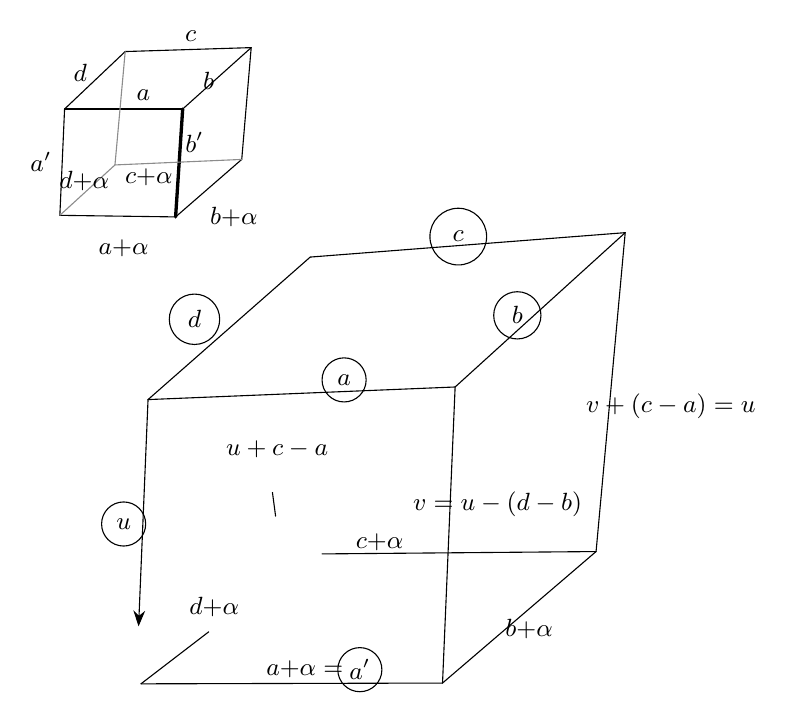
\begin{tikzpicture}[x=1mm,y=1mm,line cap=round,line join=round,font=\scriptsize]
\draw (14,-23.3) -- (29,-23.3);
\draw (29,-23.3) -- (37.7,-15.5);
\draw (21.7,-16) -- (37.7,-15.5);
\draw (21.7,-16) -- (14,-23.3);
\draw (14,-23.3) -- (13.4,-36.8);
\draw (37.7,-15.5) -- (36.5,-29.7);
\draw (13.4,-36.8) -- (28.1,-37);
\draw (28.1,-37) -- (36.5,-29.7);
\draw[very thick] (29,-23.3) -- (28.1,-37);
\draw[pencil] (21.7,-16) -- (20.4,-30.4);
\draw[pencil] (20.4,-30.4) -- (36.5,-29.7);
\draw[pencil] (13.4,-36.8) -- (20.4,-30.4);
\node[inner sep=1pt] at (30,-14) {\small $c$};
\node[inner sep=1pt] at (16,-18.7) {\small $d$};
\node[inner sep=1pt] at (24,-21.5) {\small $a$};
\node[inner sep=1pt] at (32.3,-19.7) {\small $b$};
\node[inner sep=1pt] at (11,-30) {\small $a'$};
\node[inner sep=1pt] at (30.5,-27.5) {\small $b'$};
\node[inner sep=1pt] at (16.5,-32.5) {\small $d{+}\alpha$};
\node[inner sep=1pt] at (24.7,-32) {\small $c{+}\alpha$};
\node[inner sep=1pt] at (35.5,-37) {\small $b{+}\alpha$};
\node[inner sep=1pt] at (21.5,-41) {\small $a{+}\alpha$};
\draw (24.6,-60.2) -- (63.6,-58.6);
\draw (63.6,-58.6) -- (62,-96.2);
\draw (23.7,-96.3) -- (62,-96.2);
\draw[-{Stealth[length=2mm]}] (24.6,-60.2) -- (23.4,-89);
\draw (24.6,-60.2) -- (45.2,-42.1);
\draw (45.2,-42.1) -- (85.2,-39);
\draw (63.6,-58.6) -- (85.2,-39);
\draw (85.2,-39) -- (81.5,-79.5);
\draw (62,-96.2) -- (81.5,-79.5);
\draw (46.7,-79.8) -- (81.5,-79.5);
\draw (23.7,-96.3) -- (32.3,-89.7);
\draw (40.4,-72) -- (40.8,-75);
\draw (64,-39.5) circle[radius=3.6];
\node[inner sep=1pt] at (64,-39.5) {\small $c$};
\draw (30.5,-50) circle[radius=3.2];
\node[inner sep=1pt] at (30.5,-50) {\small $d$};
\draw (71.5,-49.5) circle[radius=3];
\node[inner sep=1pt] at (71.5,-49.5) {\small $b$};
\draw (49.5,-57.7) circle[radius=2.8];
\node[inner sep=1pt] at (49.5,-57.7) {\small $a$};
\draw (21.5,-76) circle[radius=2.8];
\node[inner sep=1pt] at (21.5,-76) {\small $u$};
\draw (51.5,-94.5) circle[radius=2.8];
\node[inner sep=1pt] at (51.5,-94.5) {\small $a'$};
\node[inner sep=1pt] at (41,-66.5) {\small $u+c-a$};
\node[inner sep=1pt] at (69,-73.5) {\small $v=u-(d-b)$};
\node[inner sep=1pt] at (54,-78.3) {\small $c{+}\alpha$};
\node[inner sep=1pt] at (91,-61) {\small $v+(c-a)=u$};
\node[inner sep=1pt] at (33,-86.5) {\small $d{+}\alpha$};
\node[inner sep=1pt] at (44.5,-94.5) {\small $a{+}\alpha=$};
\node[inner sep=1pt] at (73,-89.3) {\small $b{+}\alpha$};
\end{tikzpicture}
\end{document}
